\section{peo\-Seq\-Transform$<$ EOT $>$ Class Template Reference}
\label{classpeo_seq_transform}\index{peoSeqTransform@{peoSeqTransform}}
The {\bf peo\-Seq\-Transform}{\rm (p.\,\pageref{classpeo_seq_transform})} represent a wrapper for offering the possibility of using EO derived transform operators along with the Paradis\-EO evolutionary algorithms.  


{\tt \#include $<$peo\-Seq\-Transform.h$>$}

Inheritance diagram for peo\-Seq\-Transform$<$ EOT $>$::\begin{figure}[H]
\begin{center}
\leavevmode
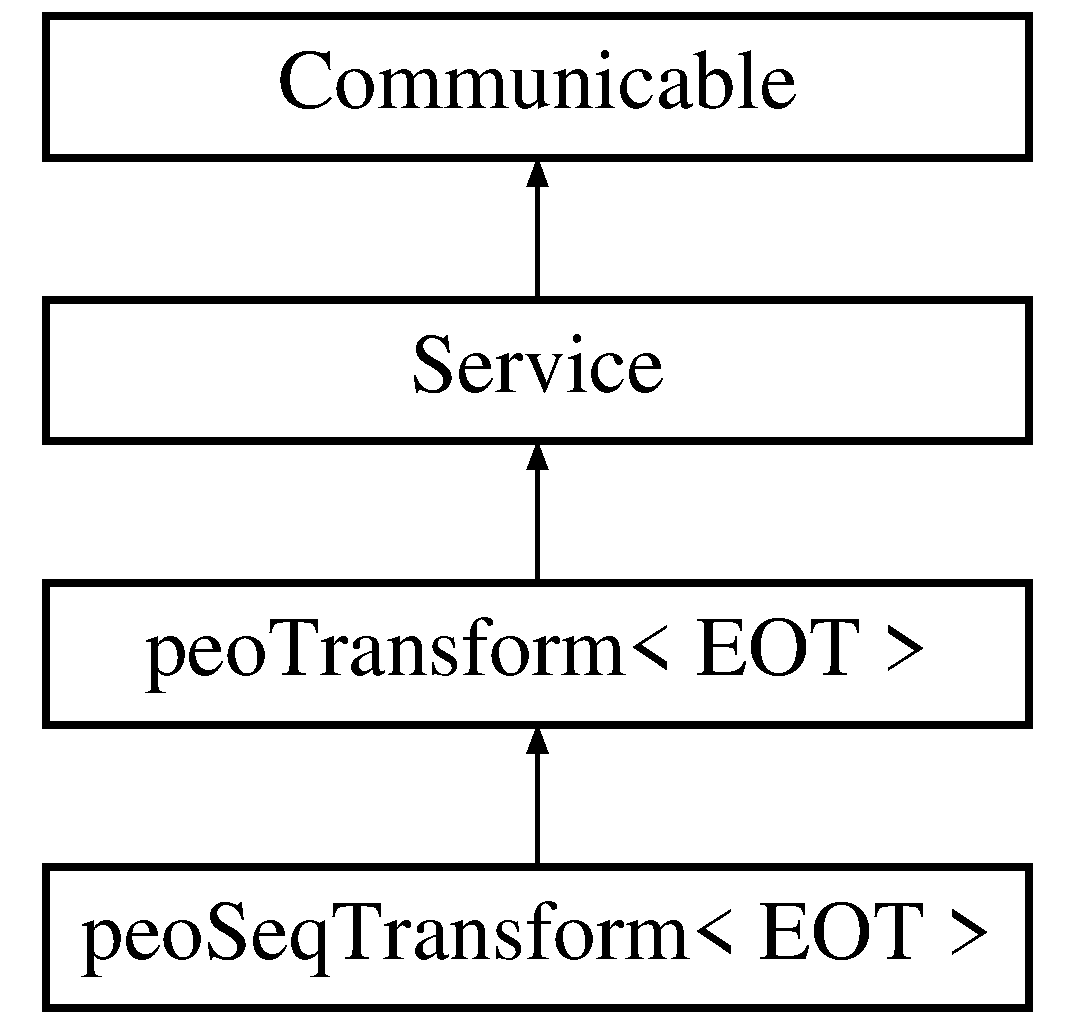
\includegraphics[height=4cm]{classpeo_seq_transform}
\end{center}
\end{figure}
\subsection*{Public Member Functions}
\begin{CompactItemize}
\item 
{\bf peo\-Seq\-Transform} (eo\-Transform$<$ EOT $>$ \&\_\-\_\-trans)
\begin{CompactList}\small\item\em Constructor function - sets an internal reference towards the specified EO-derived transform object. \item\end{CompactList}\item 
void {\bf operator()} (eo\-Pop$<$ EOT $>$ \&\_\-\_\-pop)
\begin{CompactList}\small\item\em Operator for applying the specified transform operators on each individual of the given population. \item\end{CompactList}\item 
virtual void {\bf pack\-Data} ()\label{classpeo_seq_transform_c4bf2724e9f6055f12bd169fad893be3}

\begin{CompactList}\small\item\em Interface function for providing a link with the parallel architecture of the Paradis\-EO framework. \item\end{CompactList}\item 
virtual void {\bf unpack\-Data} ()\label{classpeo_seq_transform_24e6cf15ef230ed538031b522ddd4ae6}

\begin{CompactList}\small\item\em Interface function for providing a link with the parallel architecture of the Paradis\-EO framework. \item\end{CompactList}\item 
virtual void {\bf execute} ()\label{classpeo_seq_transform_0294a2f9d6b44ec74d22eaceccdffc2b}

\begin{CompactList}\small\item\em Interface function for providing a link with the parallel architecture of the Paradis\-EO framework. \item\end{CompactList}\item 
virtual void {\bf pack\-Result} ()\label{classpeo_seq_transform_4861c61f9e46d83964ea8a156a9a3ee0}

\begin{CompactList}\small\item\em Interface function for providing a link with the parallel architecture of the Paradis\-EO framework. \item\end{CompactList}\item 
virtual void {\bf unpack\-Result} ()\label{classpeo_seq_transform_5dd029fc011eb2a810ca1140025129b1}

\begin{CompactList}\small\item\em Interface function for providing a link with the parallel architecture of the Paradis\-EO framework. \item\end{CompactList}\end{CompactItemize}
\subsection*{Private Attributes}
\begin{CompactItemize}
\item 
eo\-Transform$<$ EOT $>$ \& {\bf trans}\label{classpeo_seq_transform_ad3e16c59dd6c46dfc1baf7b88af30cf}

\end{CompactItemize}


\subsection{Detailed Description}
\subsubsection*{template$<$class EOT$>$ class peo\-Seq\-Transform$<$ EOT $>$}

The {\bf peo\-Seq\-Transform}{\rm (p.\,\pageref{classpeo_seq_transform})} represent a wrapper for offering the possibility of using EO derived transform operators along with the Paradis\-EO evolutionary algorithms. 

A minimal set of interface functions is also provided for creating the link with the parallel architecture of the Paradis\-EO framework. 



Definition at line 35 of file peo\-Seq\-Transform.h.

\subsection{Constructor \& Destructor Documentation}
\index{peoSeqTransform@{peo\-Seq\-Transform}!peoSeqTransform@{peoSeqTransform}}
\index{peoSeqTransform@{peoSeqTransform}!peoSeqTransform@{peo\-Seq\-Transform}}
\subsubsection{\setlength{\rightskip}{0pt plus 5cm}template$<$class EOT$>$ {\bf peo\-Seq\-Transform}$<$ EOT $>$::{\bf peo\-Seq\-Transform} (eo\-Transform$<$ EOT $>$ \& {\em \_\-\_\-trans})}\label{classpeo_seq_transform_3b8e4ed19d9458938eb669d83a53c626}


Constructor function - sets an internal reference towards the specified EO-derived transform object. 

\begin{Desc}
\item[Parameters:]
\begin{description}
\item[{\em eo\-Transform$<$}]EOT $>$\& \_\-\_\-trans - EO-derived transform object including crossover and mutation operators. \end{description}
\end{Desc}


Definition at line 70 of file peo\-Seq\-Transform.h.

\subsection{Member Function Documentation}
\index{peoSeqTransform@{peo\-Seq\-Transform}!operator()@{operator()}}
\index{operator()@{operator()}!peoSeqTransform@{peo\-Seq\-Transform}}
\subsubsection{\setlength{\rightskip}{0pt plus 5cm}template$<$class EOT$>$ void {\bf peo\-Seq\-Transform}$<$ EOT $>$::operator() (eo\-Pop$<$ EOT $>$ \& {\em \_\-\_\-pop})}\label{classpeo_seq_transform_1ba63536abb6c4e1c369e0b7e066872e}


Operator for applying the specified transform operators on each individual of the given population. 

\begin{Desc}
\item[Parameters:]
\begin{description}
\item[{\em eo\-Pop$<$}]EOT $>$\& \_\-\_\-pop - population to be transformed by applying the crossover and mutation operators. \end{description}
\end{Desc}


Definition at line 75 of file peo\-Seq\-Transform.h.

References peo\-Seq\-Transform$<$ EOT $>$::trans.

The documentation for this class was generated from the following file:\begin{CompactItemize}
\item 
peo\-Seq\-Transform.h\end{CompactItemize}
